\documentclass[10pt,a4paper]{article}
\usepackage[T1]{fontenc}\usepackage[utf8]{inputenc}\usepackage[margin=20mm]{geometry}\usepackage{graphicx,tabularx,booktabs,array,fancyhdr,enumitem}
\pagestyle{fancy}\fancyhf{}\lhead{IIT Indore}\rhead{Machine Learning in Forex}\cfoot{\thepage}\setlength{\headheight}{15pt}\setlength{\parindent}{0pt}\setlength{\parskip}{5pt}\setlist[itemize]{nosep,leftmargin=*}\begin{document}
\thispagestyle{empty}\begin{center}\vspace*{14mm}
\section*{Machine Learning in Forex}
Cumulative B.Tech Project Report\par
{\centering
\includegraphics[width=\linewidth,height=38mm,keepaspectratio]{figures/1-IITI_Logo.png}\par}
Department of Physics $\cdot$ Indian Institute of Technology Indore\par
\subsection*{Prince Kumar}
Engineering Physics $\cdot$ Roll No. 230051013\par
\subsection*{Supervisors}
Prof. Raghunath Sahu and Dr. Kalindi C. Pradhan\par
November 2026\par
\end{center}
\clearpage
\section*{Abstract}
How much of a currency forecast survives the decision to trade? This project follows that question from daily exchange-rate models to minute-level execution and a shared portfolio of equities. On 681 held-out observations, the daily LSTM predicted 378 USD/INR directions correctly. Simply predicting up achieved 375. On EUR/USD, validation fine-tuning raised the correct count from 347 to 363. In a separate 65-session EUR/USD simulation, the trading strategy gained 2.28\% while a passive euro holding lost 1.59\% by exact compounding.\par
The equity extension used 100 Indian and 95 US stock files. It compared a forecast threshold with a learned trading policy, then combined technical strategies and evolved rules in a shared account. The best saved Indian and US portfolio configurations returned 250.87\% and 12.50\% over their respective historical periods. A final policy trained on five strategy signals earned 4.02\% on its 95-stock US test. Different periods, position limits and cost assumptions restrict comparisons across these experiments.\par
\subsection*{Contents}
\begin{tabularx}{\linewidth}{@{}p{0.75\linewidth}X@{}}\toprule
Section & Page\\\midrule
Introduction & 3\\
Literature Review and Research Gaps & 4\\
1   Forex data and forecasting baselines & 5\\
1.1 Building a daily return forecast & 6\\
2   Daily LSTM and corrected direction scores & 7\\
2.1 How BigMoveAwareLoss weights forecast errors & 8\\
3   EUR/USD execution and the passive benchmark & 9\\
3.1 Calibrating stops, targets and position size & 10--11\\
4   Auditing the one-minute equity data & 12\\
5   Feature construction and indicator screening & 13\\
6   Trading the intraday LSTM forecasts & 14\\
7   Parameter search and genetic programming & 15\\
8   Shared-capital Indian equity portfolio & 16--17\\
9   US equity portfolio & 18\\
9.1 Shared portfolios versus buy-and-hold & 19\\
9.2 Trading charges in the top-10 portfolios & 20\\
10  Reinforcement learning over strategy signals & 21\\
11  Future Plans & 22\\
12  Conclusions and next experiments & 23\\
References and experimental records & 24\\
\bottomrule\end{tabularx}\par
\clearpage
\section*{Introduction}

A correct exchange-rate forecast can still lead to a losing trade. The predicted move may be too small to cover trading costs, or the price may hit a stop-loss before moving in the expected direction. This project began with two questions. How accurately can a model predict the next daily movement in USD/INR and EUR/USD? Under what conditions does acting on a forecast improve the outcome for a trader?

I first compared statistical and machine-learning forecasts against simple baselines, including using the latest exchange rate as the next prediction. I evaluated both price error and directional accuracy, then used a historical EUR/USD simulation to examine how entry thresholds, position sizing and exit rules affected returns and drawdown.

I extended the investigation to minute-level Indian and US equity data, where trading decisions also depend on the quality of individual price bars and the capital available across stocks. I tested trading rules with explicit entry conditions and trained a reinforcement-learning policy to act on their signals. The policy rewarded portfolio growth and penalized increases in drawdown. Evaluating it on a later period allowed me to examine how it behaved on prices it had not seen during training.

\clearpage
\section*{Literature Review and Research Gaps}
Several published studies examine machine learning for currency markets~[1--6].
\begin{itemize}
  \item \textbf{Forecasting approaches.} Babu and Geethanjali~[3] classify forex trends with machine learning techniques. Fisichella and Garolla~[1] show that deep learning applied to technical indicators achieves directional accuracy above simple moving-average baselines on EUR/USD. Huang~[2] formulates currency trading as a sequential decision problem and applies deep Q-networks to generate buy and sell signals. Giacinto et al.~[5] stack an LSTM regressor under a reinforcement-learning policy for high-frequency FX trading. Grover et al.~[6] evolve an ensemble of machine-learning models with a genetic algorithm, optimising trading rules jointly with model selection.
  \item \textbf{Macroeconomic integration.} Most papers use only technical features because macroeconomic data arrives at lower frequency than price ticks. Sharma and Pradhan~[4] combine macro and market features, reaching around $60.9\%$ directional accuracy on EUR/USD; however, their simulation produced a $-16\%$ return over the same period---demonstrating that higher prediction accuracy does not guarantee profitable trading.
\end{itemize}

\subsection*{Research gaps addressed by this project}
\begin{enumerate}[leftmargin=1.5cm, itemsep=2pt]
  \item \textbf{The forecast-to-trade gap.} Existing papers typically report prediction accuracy or simulated returns in isolation. This project tracks the same daily LSTM signals through daily close-to-close backtesting, granularity-mismatch correction, live one-minute simulation, and a shared-capital portfolio layer---documenting where accuracy translates into trading edge and where it does not.
  \item \textbf{Post hoc explainability of RL policy inputs.} No reviewed study applies feature-attribution methods such as SHAP to explain which macro variables drive a reinforcement-learning agent's decisions during specific market events such as central bank rate decisions or intervention operations.
\end{enumerate}

\clearpage
\section*{1. Forex data and forecasting baselines}
The initial experiments ask whether yesterday's observations help forecast the next exchange-rate move. USD/INR quotes rupees per dollar; EUR/USD quotes dollars per euro. For each pair, a positive return denotes appreciation of the base currency.\par
\begin{itemize}\item \textbf{Data and predictors.} The FRED inputs include both target currencies, the yen exchange rate, the federal funds rate and the US ten-year Treasury yield. The training notebook aligns observations by date and drops incomplete rows before constructing chronological splits.\end{itemize}
\begin{itemize}\item \textbf{Models.} Persistence and a three-day moving average provide training references. The notebook also fits ARIMA, linear models and neural networks. Technical inputs summarize moving averages, momentum and dispersion; temporal features extend the feed-forward model.\end{itemize}
\begin{itemize}\item \textbf{Evaluation.} Mean absolute error (MAE) and root mean squared error (RMSE) measure price-level error. Directional accuracy asks whether the model got the sign of the move right.\end{itemize}
\begin{tabularx}{\linewidth}{@{}p{0.34\linewidth}XXX@{}}\toprule
USD/INR test model & MAE & RMSE & Direction\\\midrule
Base deep MLP & 1.8872 & 1.9150 & 44.93\%\\
MLP + technical features & 0.1917 & 0.2553 & 52.21\%\\
MLP + technical and temporal features & 0.1558 & 0.2395 & 52.30\%\\
\bottomrule\end{tabularx}\par
Source: model\_results.json, metrics.test. Direction was scored on 690, 680 and 675 observations respectively. ARIMA(2, 0, 1) has a separate validation record: MAE 1.1895, RMSE 1.5280 and direction 53.85\% (371/689).\par
{\centering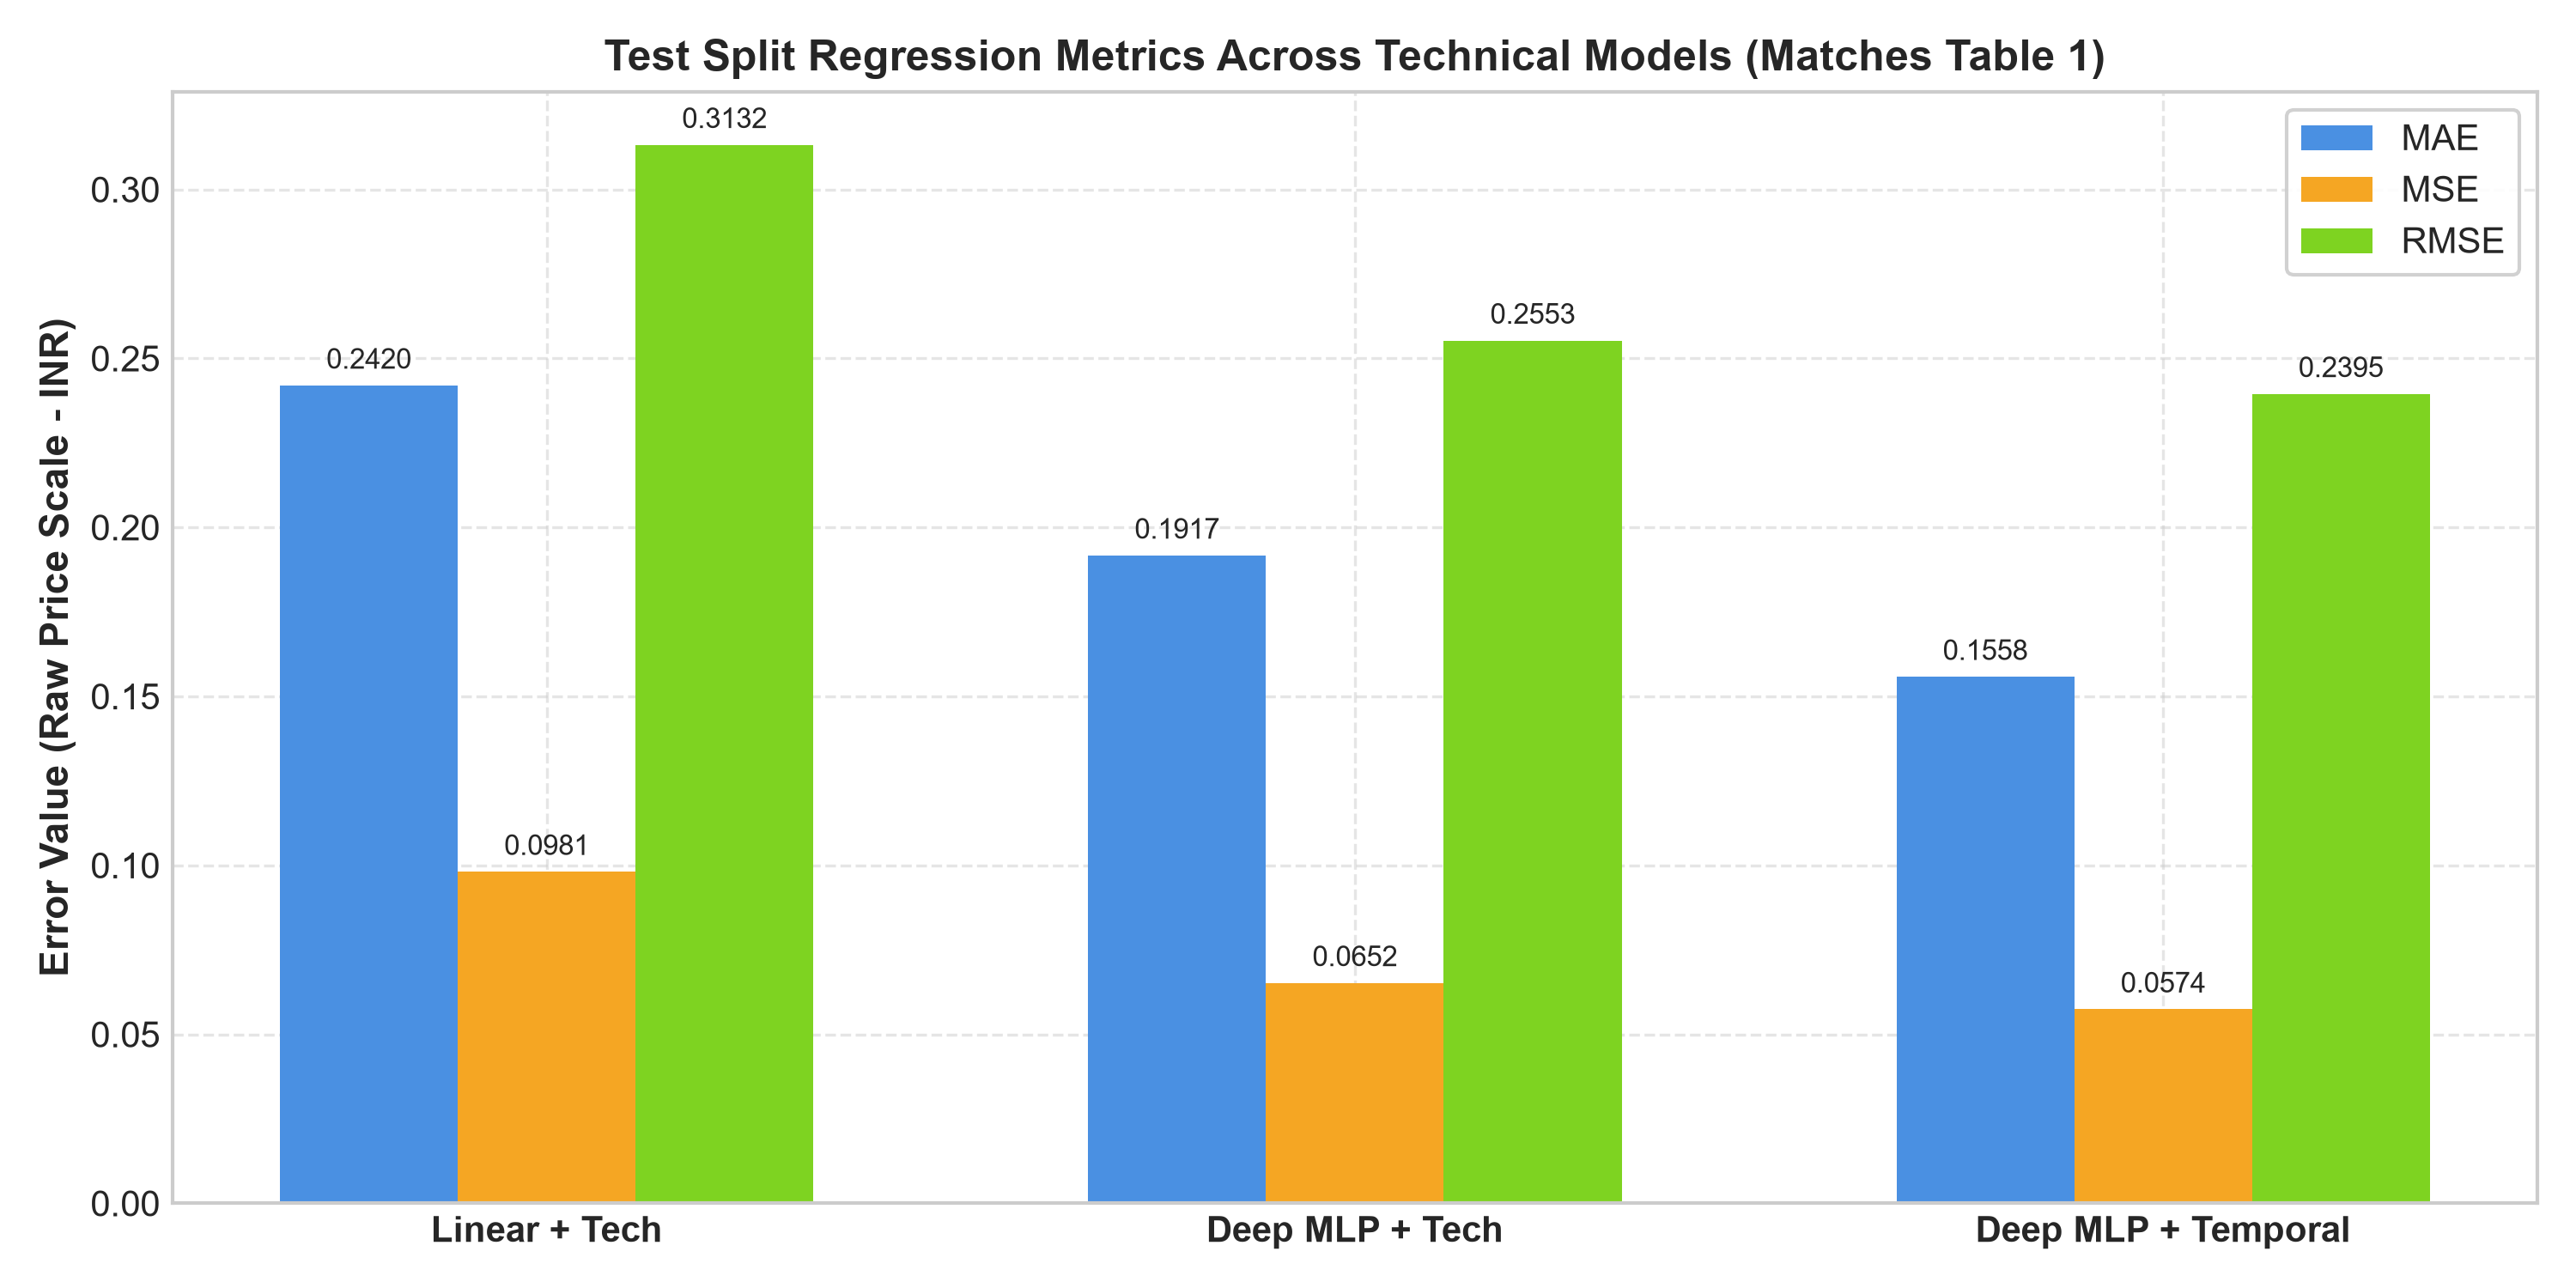
\includegraphics[width=\linewidth,height=58mm,keepaspectratio]{figures/3-evaluation-regression-test.png}\par}
{\small\itshape Figure 1. Saved evaluation plot for three technical-feature models. Adding temporal features reduced price error. The last two directional scores cover different observation counts.\par}
This distinction motivated the shift from predicting a price level to learning daily returns. The technical-analysis study of Fisichella and Garolla [1] provided a related formulation for the forex forecasting question.\par
\clearpage
\section*{1.1 Building a daily return forecast}
A model can track the level of an exchange rate closely while getting tomorrow's direction wrong. The base USD/INR MLP had a test RMSE of 1.9150 rupees per dollar. With technical and temporal inputs, RMSE fell to 0.2395, while directional accuracy reached 52.30\%. The eligible test windows differed slightly across models.\par
\subsection*{What one training example contains}
At forecast time the model reads ten consecutive observations. Each row contains 23 features. A single LSTM layer with 32 hidden units summarizes the window, and a linear output maps the last hidden state to one predicted log return. A positive next-day log return means the quoted pair closed higher.\par
\textbf{5 market inputs.} The target exchange rate, two other currency quotes, the federal funds rate and the US ten-year yield give the model cross-market context.\par
\textbf{10 trend inputs.} Simple and exponential moving averages at 5, 10, 30, 50 and 100 days describe trends over different horizons.\par
\textbf{8 momentum and risk inputs.} RSI, the current log return, three Bollinger-band values, rolling volatility and two range proxies describe recent moves and their variability.\par
\subsection*{How the model is evaluated}
The feature and target scalers use training observations. The same scales are applied to validation and test windows. Forecasts are converted back to log returns before scoring direction against zero. Keeping this distinction matters because zero on the standardized scale represents the training mean.\par
Sources: train.ipynb, daily currency data loaders and LSTM training cells. BTP Executive Summary, pp. 1--3.\par
\subsection*{Data sources and splits}
\begin{itemize}
  \item \textbf{Data sources.} Historical daily rates from FRED (Federal Reserve H.10) covering over 6,800 trading days; live ticker data from Yahoo Finance (\texttt{EURUSD=X}, \texttt{INR=X}, \texttt{JPY=X}, \texttt{\textasciicircum TNX}). US bond markets close on US holidays while forex markets stay open; missing rows are forward-filled (\texttt{ffill}) so the feature matrix stays continuous without look-ahead.
  \item \textbf{Strictly chronological split.} Train: $80\%$ ($\approx5{,}434$ days); Validation: $10\%$ ($\approx680$ days); Test: $10\%$ ($\approx681$ days). \texttt{StandardScaler} is fitted on the training window only and applied to validation and test without refitting.
  \item \textbf{Why log returns rather than price levels.} A move of $+1.00$ on USD/INR represented $2.2\%$ in 2010 (rate $\approx45$) but only $1.2\%$ in 2026 (rate $\approx83$). Models trained on raw levels overfit to the absolute scale and fail on new price regimes. Log returns $y_t = \ln(C_{t+1}/C_t)$ remain near zero with stable variance across decades and are additive across time steps.
  \item \textbf{Why regression rather than 3-class classification.} An intermediate experiment labelled each day Buy ($>\!+\tau$), Sell ($<\!-\tau$), or Hold ($[-\tau,+\tau]$). The classes were heavily imbalanced toward Hold with any small $\tau$, and the label discarded return magnitude---which is required to compute stop distances and position sizes. Predicting a continuous log return directly resolves both problems.
\end{itemize}
\clearpage
\section*{2. Daily LSTM and corrected direction scores}
\begin{itemize}\item \textbf{Input.} Each sequence contains ten daily observations. The forex configuration combines 23 market and technical features. A single LSTM layer with 32 hidden units passes its final state to a linear return prediction.\end{itemize}
\begin{itemize}\item \textbf{Objective.} The loss weights squared errors more heavily for large realized moves and adds a sign-mismatch penalty. The sign operation has zero gradient almost everywhere. Magnitude weighting supplies the useful gradient; a controlled comparison would be needed to attribute a gain to loss design.\end{itemize}
\begin{itemize}\item \textbf{Evaluation rule.} For each forecast, compare the predicted and realized log return with zero. A flat return counts as up under the project convention. Comparing both values with yesterday's return instead measures whether they lie on the same side of yesterday's move.\end{itemize}
\begin{tabularx}{\linewidth}{@{}p{0.34\linewidth}XXX@{}}\toprule
Test series & Correct / total & Direction & Return RMSE\\\midrule
USD/INR & 378 / 681 & 55.51\% & 0.00263\\
EUR/USD before fine-tuning & 347 / 681 & 50.95\% & 0.00423\\
EUR/USD after fine-tuning & 363 / 681 & 53.30\% & 0.00423\\
NIFTY 50 index & 387 / 854 & 45.32\% & 0.00791\\
S\&P 500 index & 1,111 / 2,470 & 44.98\% & 0.01201\\
\bottomrule\end{tabularx}\par
{\centering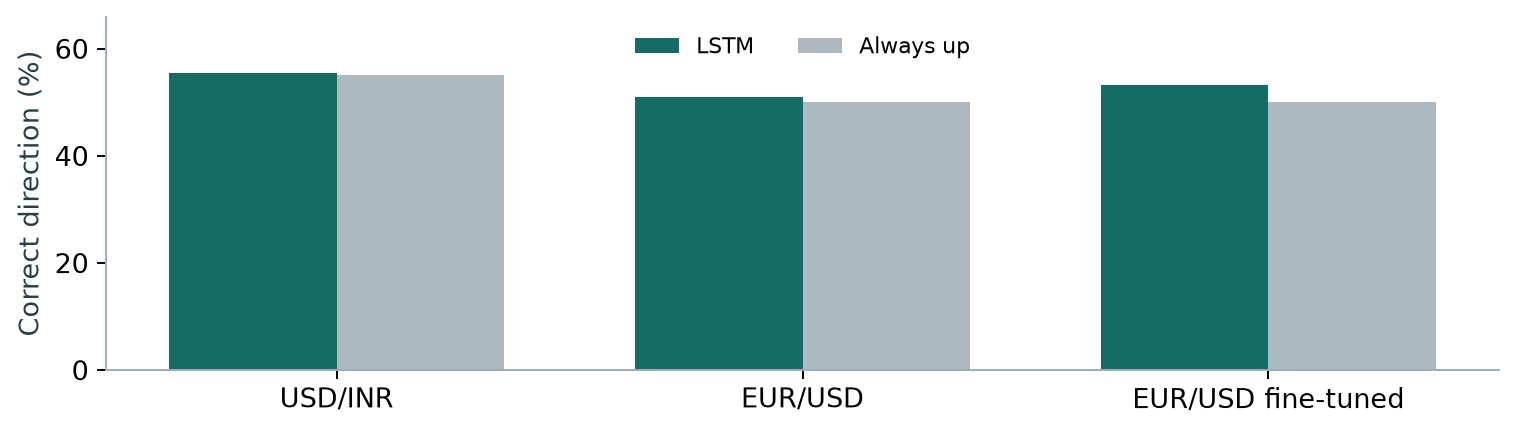
\includegraphics[width=\linewidth,height=51mm,keepaspectratio]{figures/4-accuracy.png}\par}
{\small\itshape Figure 2. Currency forecasts and the always-up rule on the same test observations. USD/INR gained three correct calls over the baseline. Fine-tuned EUR/USD gained 22.\par}
{\centering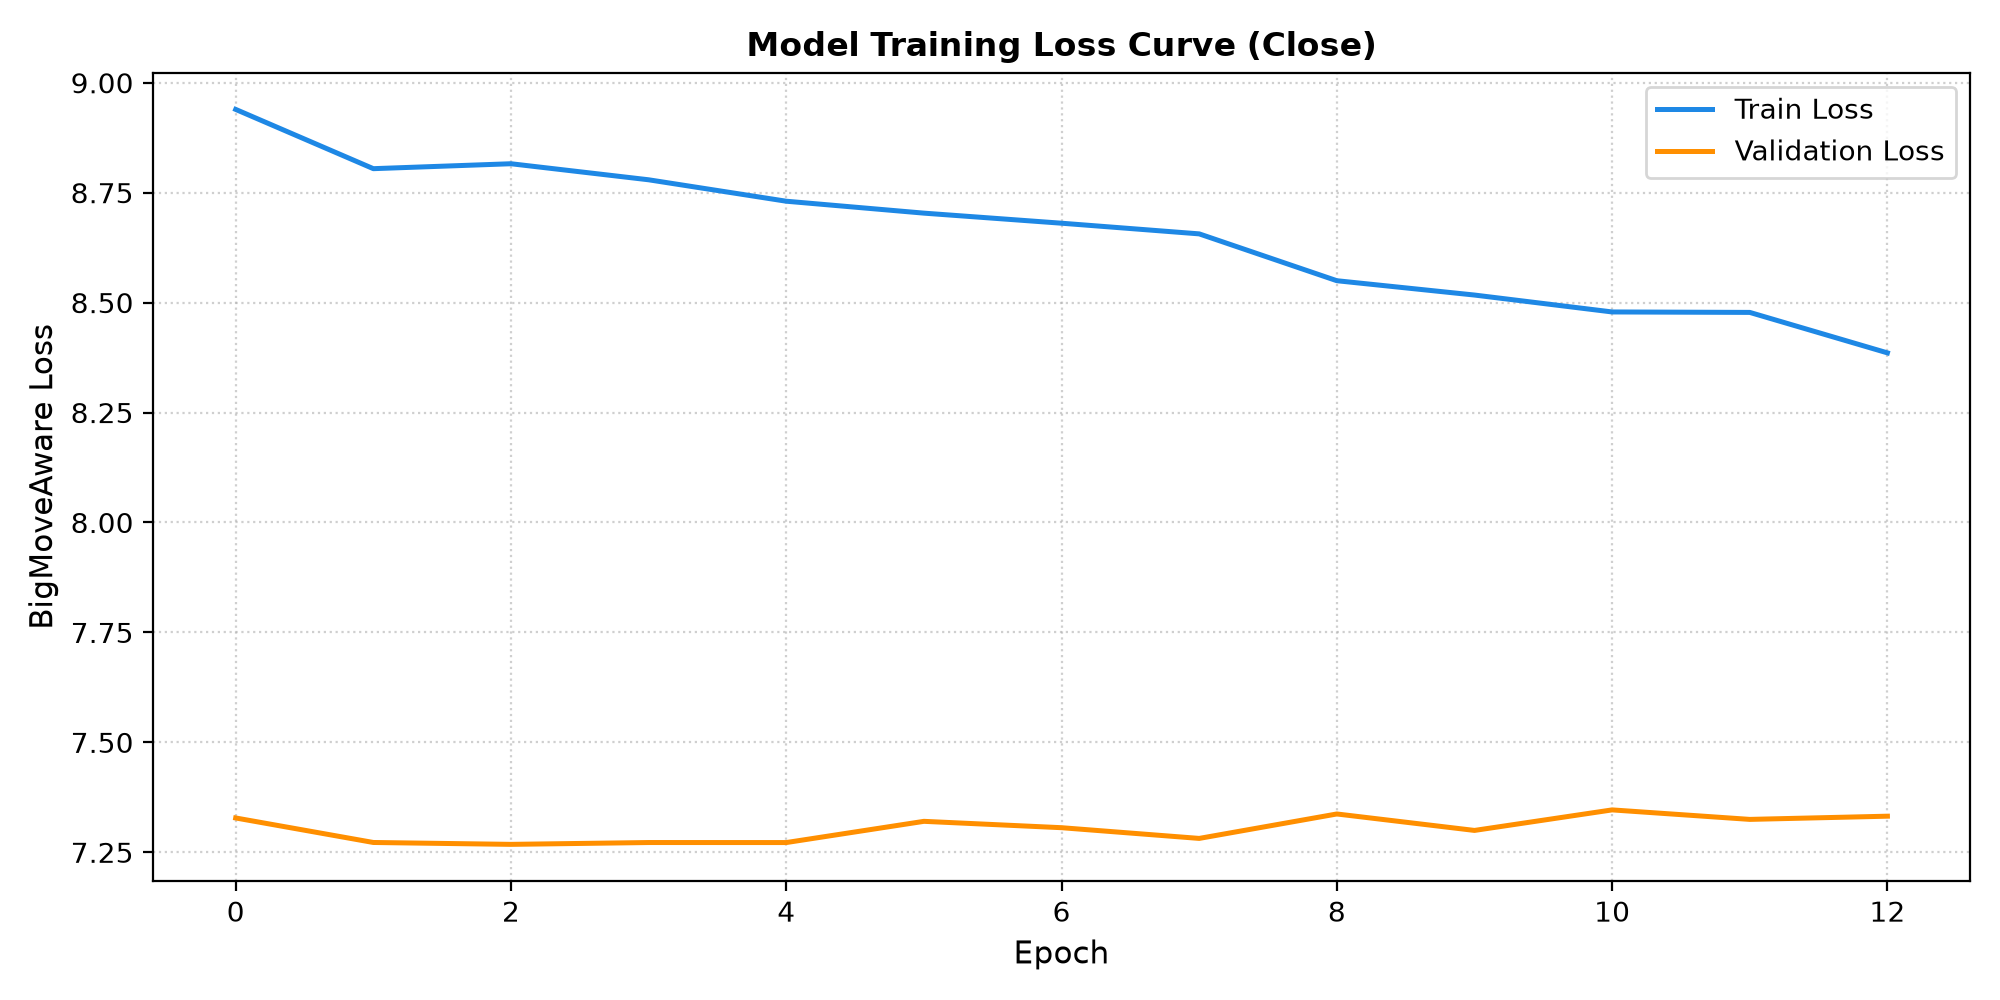
\includegraphics[width=\linewidth,height=31mm,keepaspectratio]{figures/4-1_training_loss.png}\par}
{\small\itshape Figure 3. Training and validation loss from the NIFTY 50 LSTM run. Its test direction score was 45.32\%.\par}
Validation fine-tuning added 16 correct EUR/USD predictions. The two index experiments gave lower hit rates. These directional results measure one decision per forecast; trading returns additionally depend on the size, timing and cost of each position.\par
\subsection*{Cross-asset strategy backtest summary}
The same LSTM + BigMoveAwareLoss + GA pipeline (\texttt{GeneralTrainer}) was applied without manual re-tuning to all four assets. The table below adds backtested strategy performance to the directional accuracy results.
\begin{tabularx}{\linewidth}{@{}p{0.28\linewidth}XXXXXX@{}}
\toprule
Asset & Direction & MAE & RMSE & Strategy Sharpe & Calmar\\\midrule
USD/INR (Forex) & 55.51\% & 0.00181 & 0.00263 & 2.10 & 4.52\\
EUR/USD (Forex) & 53.30\% & 0.00310 & 0.00423 & 3.73 & 18.48\\
Nifty 50 & 45.32\% & 0.00586 & 0.00791 & 3.87 & 11.82\\
S\&P 500 & 44.98\% & 0.00827 & 0.01201 & 3.91 & 18.94\\
\bottomrule
\end{tabularx}\par
{\small\itshape Sharpe and Calmar are from the backtested strategy run on each asset's held-out test period. EUR/USD Sharpe and Calmar correspond directly to the fine-tuned test results (Section~3.1). Nifty and S\&P metrics are from the \texttt{GeneralTrainer} daily strategy run on those indices. Direction is scored against zero (stationary mean) with flat returns counted as up; the always-up baseline scores 55.07\% on USD/INR and 50.07\% on EUR/USD over the same 681 observations.}\par
\clearpage
\section*{2.1 How BigMoveAwareLoss weights forecast errors}
Most daily returns are small. An estimate near the mean can therefore achieve a modest average squared error while missing the days with large price moves. The project introduced BigMoveAwareLoss to give those observations more influence during training.\par
\subsection*{The objective used in the notebook}
Let z be the realized return in training-standard-deviation units after centering, and p the prediction on the same scale. Set B to 1 when $|z|$ is at least 1.5 and to 0 otherwise. The notebook averages the following loss over each batch.\par
\[ L=(1+2|z|+4B)(p-z)^2+0.5(|z|+2B)\,\mathbf{1}_{pz<0}. \]
\textbf{Magnitude term.} Squared error receives a weight of 1 + 2|z|. Crossing the large-move threshold adds another 4.\par
\textbf{Direction term.} When p and z have opposite signs, the loss adds half of |z|, plus one more unit on a large move. A prediction of zero incurs no sign penalty.\par
\subsection*{Worked example}
For a realized z of +2, the squared-error weight is 9. A forecast of +1 incurs a loss of 9. A forecast of -1 incurs 81 from squared error and 2 from the sign penalty, bringing the loss to 83. The sign term changes the reported loss, but its hard sign operation has zero gradient almost everywhere. The weighted squared error supplies the gradient that updates the model.\par
The corrected USD/INR test score was 378/681, versus 375/681 for always predicting up. Isolating the effect of the custom loss requires training the same architecture on the same split with ordinary MSE.\par
Sources: train.ipynb, BigMoveAwareLoss.forward and both currency loss configurations. BTP Executive Summary, pp. 3--4.\par
\clearpage
\section*{3. EUR/USD execution and the passive benchmark}
\begin{itemize}\item \textbf{Backtesting engine (\texttt{AdvancedProfitCalculator}).} Trades risk a fixed percentage of equity per position. The stop loss sets the worst-case loss; take profit equals stop loss times the reward-to-risk ratio. A 1-pip (\$0.0001) fee is deducted on every entry and exit. An unoptimised baseline with default rules (SL$=0.40\%$, RRR$=2.0$, threshold$=0.01\%$) turned \$10{,}000 into \$19{,}035.45 on the validation period (+26.94\% CAGR, max drawdown $-13.81\%$, Sharpe 1.54).\end{itemize}
\begin{itemize}\item \textbf{Strategy.} The forex genetic algorithm searched signal thresholds, stops, profit targets and sizing. The daily validation search used 40 individuals and 25 generations. A 0.20\% stop could be crossed intraday even on a day that ultimately closed in the predicted direction. The later execution simulation used wider excursion-based stops and periodic recalibration.\end{itemize}
\begin{itemize}\item \textbf{Data resolution.} The execution code requests EURUSD=X bars from Yahoo Finance. Its historical-data path can forward-fill hourly or five-minute bars onto a one-minute grid. A minute timestamp therefore does not establish that every intraminute price move was observed.\end{itemize}
\begin{itemize}\item \textbf{Benchmark.} Start with USD 10,000 and maintain an unleveraged long EUR position through all 65 evaluated daily returns, including the strategy's 20 idle sessions. The reference is the EUR/USD spot series in the simulation. It applies no trading signal or financing adjustment.\end{itemize}
\begin{tabularx}{\linewidth}{@{}p{0.34\linewidth}XX@{}}\toprule
27 July--23 October 2026 & Ending USD & Period return\\\midrule
LSTM trading strategy & 10,228.30 & +2.28\%\\
Passive euro, exact compounding & 9,841.44 & -1.59\%\\
Passive euro, original simulator ledger & 9,838.73 & -1.61\%\\
\bottomrule\end{tabularx}\par
{\centering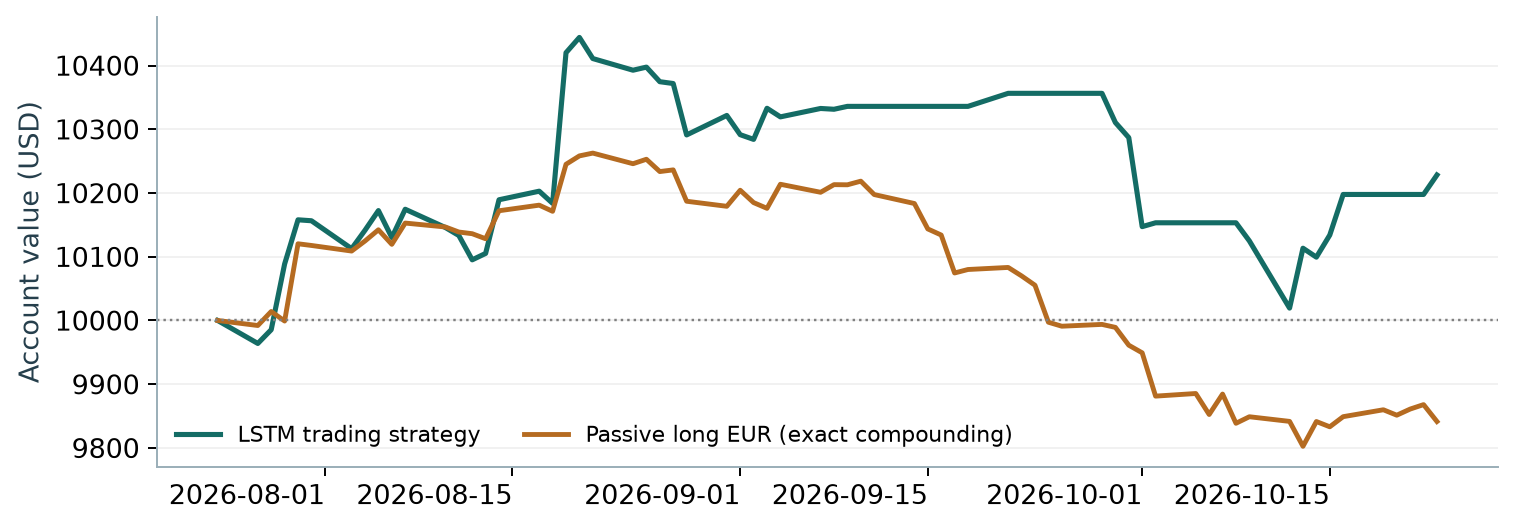
\includegraphics[width=\linewidth,height=52mm,keepaspectratio]{figures/5-eur-benchmark.png}\par}
{\small\itshape Figure 4. Equity from the trade ledger and the passive euro holding reconstructed from the same daily returns. Both start at USD 10,000 before the first evaluated return.\par}
The ledger multiplies by (1 + daily log return); exact currency compounding multiplies by exp(daily log return). The strategy finished 3.87 percentage points above the exact reference. Its maximum recorded drawdown was -4.07\%. The 22 wins averaged USD 46.25, the 23 losses averaged USD 34.32 in magnitude. Annualizing +2.28\% over 65 sessions at 252 sessions per year gives +9.15\%.\par
\clearpage
\section*{3.1 Calibrating stops, targets and position size}
A return forecast supplies a direction. The trading rule must also decide when to enter, how much capital to risk and when to exit. The EUR/USD experiment searched these decisions jointly on validation data using 40 candidate rules over 25 generations. Fitness was annualized growth divided by the absolute maximum drawdown.\par
\textbf{Exit rules.} The search allowed stops from 0.10\% to 1.20\% and reward-to-risk ratios from 1 to 3.5. It selected a 0.20\% stop and a 3.5 ratio, implying a 0.70\% profit target.\par
\textbf{Entry and exposure.} The selected configuration used a zero signal threshold, risked 2.696\% of equity per trade and capped leverage at 5 times equity. The search assumed one pip of transaction friction.\par
{\centering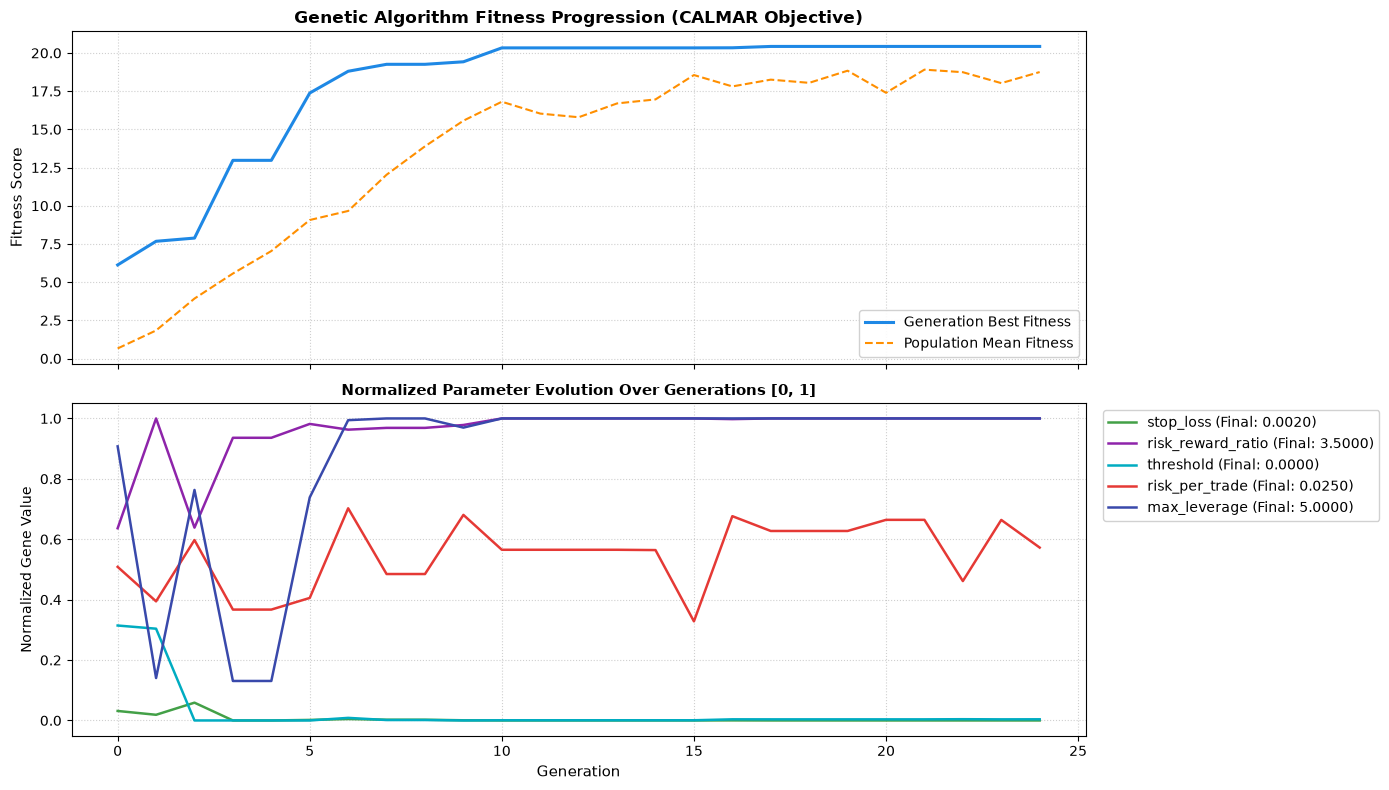
\includegraphics[height=52mm,width=\linewidth,keepaspectratio]{figures/ga-convergence.png}\par}
Validation fitness rose from 6.12 to 20.43 during the search. The curve measures selection on validation data.\par
\subsection*{Why the execution rules changed}
A long trade can fall 0.20\% after entry, hit its stop, and still close the day above its entry price. Daily closing prices hide that sequence. The execution study widened the stop range to 0.45--0.80\% and fine-tuned the model every ten sessions. Over 65 sessions it recorded 22 wins and 23 losses. Average wins of USD 46.25 exceeded average losses of USD 34.32, leaving a positive return despite winning fewer than half the trades.\par
Source: BTP Executive Summary, pp. 4--6. The preceding section details the simulation's bar resolution and passive benchmark.\par
\subsection*{Full daily test-set backtest results (681 trading days)}
The table below summarises EUR/USD performance at three evaluation stages on the held-out daily test period. The GA was fitted on validation data only; test data were never touched during parameter search or model training.
\begin{tabularx}{\linewidth}{@{}p{0.36\linewidth}XXXXX@{}}
\toprule
EUR/USD configuration & Net return & CAGR & Max DD & Sharpe & Calmar\\\midrule
Unoptimised baseline (val) & +90.35\% & +26.94\% & $-13.81\%$ & 1.54 & --\\
GA-evolved fitness target (val) & -- & +181.67\% & $-8.89\%$ & 4.34 & 20.43\\
GA params, initial LSTM (test) & +518.59\% & +96.27\% & $-9.73\%$ & 3.27 & 9.90\\
GA params, fine-tuned LSTM (test) & +704.39\% & +116.30\% & $-6.29\%$ & 3.73 & 18.48\\
Buy-and-hold benchmark (test) & +6.99\% & -- & -- & -- & --\\
\bottomrule
\end{tabularx}\par
Starting capital was \$10{,}000 in all cases. The initial test run (\$10{,}000$\to$\$61{,}858.97) executed 650 trades at a 49.85\% win rate; profit factor was 1.61 and trade expectancy \$79.78 (Sortino: 13.26). Fine-tuning on the validation data before the test period raised final equity to \$80{,}439.08. The Calmar ratio improved from 9.90 to 18.48, reflecting lower drawdown alongside higher return. Strategy alpha versus buy-and-hold on the test period was +511.60 percentage points.
These are daily close-to-close backtests. Section~3 documents the separate live simulation on one-minute bars, which reveals the execution gap: the tight 20-pip daily stop-loss is too small to survive intraday noise, so it was widened to 45--80\,pips for minute-level trading.\par
\clearpage
\section*{4. Auditing the one-minute equity data}
Historical equity data came from Kaggle, with FYERS API updates for recent observations. The source directories contain 100 Indian stock files and 95 US files. Each stock has its own start date and observation history.\par
\begin{itemize}\item \textbf{Build the expected calendar.} The EDA notebook maps timestamps to scheduled sessions and compares observed rows with expected tradable minutes. A holiday, a date before a stock's first observation and an absent bar in the middle of a session require different treatment.\end{itemize}
\begin{itemize}\item \textbf{Locate missing runs.} The Indian missing-run summary contains 36,340 runs covering 102,724 minutes across its 97 stock rows. Of those runs, 27,611 were single missing minutes. HAL alone had 7,788 runs, with one interruption lasting 227 minutes.\end{itemize}
\begin{itemize}\item \textbf{Repair eligible short gaps.} ABB was missing 09:30--09:31 on 13 March 2015. A two-bar repair requires two valid observations on either side in the same session. Each field is averaged over those four surrounding bars; both missing rows receive that field's mean.\end{itemize}
\begin{itemize}\item \textbf{Preserve longer interruptions.} ABB's gap at 09:15--09:34 on 16 March spans 20 minutes. It exceeds the three-minute limit and remains missing. The feature pipeline restarts its rolling history after the break.\end{itemize}
{\centering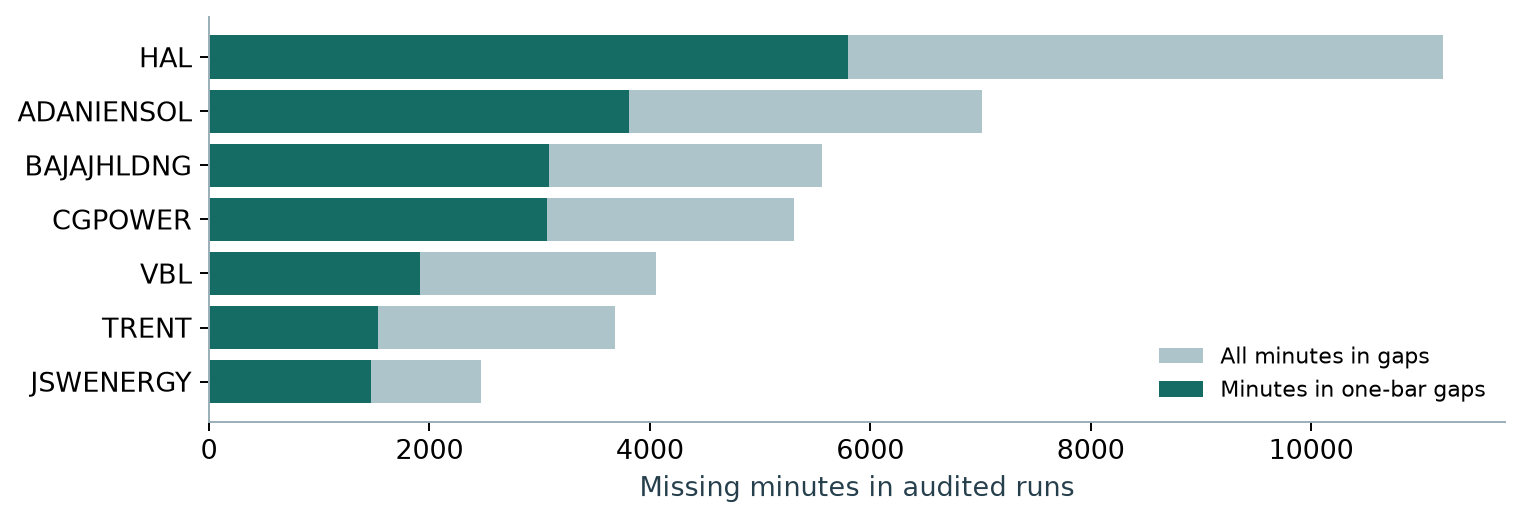
\includegraphics[width=\linewidth,height=65mm,keepaspectratio]{figures/6-gap-audit.png}\par}
{\small\itshape Figure 5. Seven stocks with the most missing minutes in the Indian run-level audit. The darker segment counts isolated missing minutes; the balance belongs to longer runs.\par}
The short-gap repair uses future observations. The pipeline marks repaired rows. The quantitative strategy loader excludes imputed bars and masks downstream indicators affected within the segment. A causal-filling comparison remains relevant for the forecasting branch.\par
\clearpage
\section*{5. Feature construction and indicator screening}
\begin{itemize}\item \textbf{Segment before rolling.} A session change, an invalid observation or a timestamp jump creates a new segment. The first return and rolling windows after a break require fresh observations. This prevents an overnight price change from being treated as a one-minute return.\end{itemize}
\begin{itemize}\item \textbf{Reuse prepared data.} Per-stock Parquet files retain OHLCV values, validity and imputation flags, segment IDs and derived columns. The downstream LSTM reads a seven-feature subset; the strategy engines consume their respective indicators.\end{itemize}
\begin{tabularx}{\linewidth}{@{}p{0.26\linewidth}X@{}}\toprule
Feature family & Examples and application\\\midrule
Price movement and trend & Simple/log returns, SMA, EMA, MACD and fitted trend slope\\
Range and momentum & RSI, Bollinger bands and Donchian channels for reversal or breakout signals\\
Volume and volatility & VWAP, relative volume, OBV and rolling volatility. Optional daily GARCH uses earlier sessions, with 60--252 returns of history.\\
\bottomrule\end{tabularx}\par
\subsection*{Did additional indicators improve the forecast?}
A separate NIFTY 50 study used 209,888 five-minute bars. A ridge model predicted 5-, 15- and 60-minute returns over three expanding-window folds. Of the candidate feature pairs, 114 had absolute training Spearman correlation of at least 0.95. A training-only redundancy screen retained 32 of the 61 indicators.\par
{\centering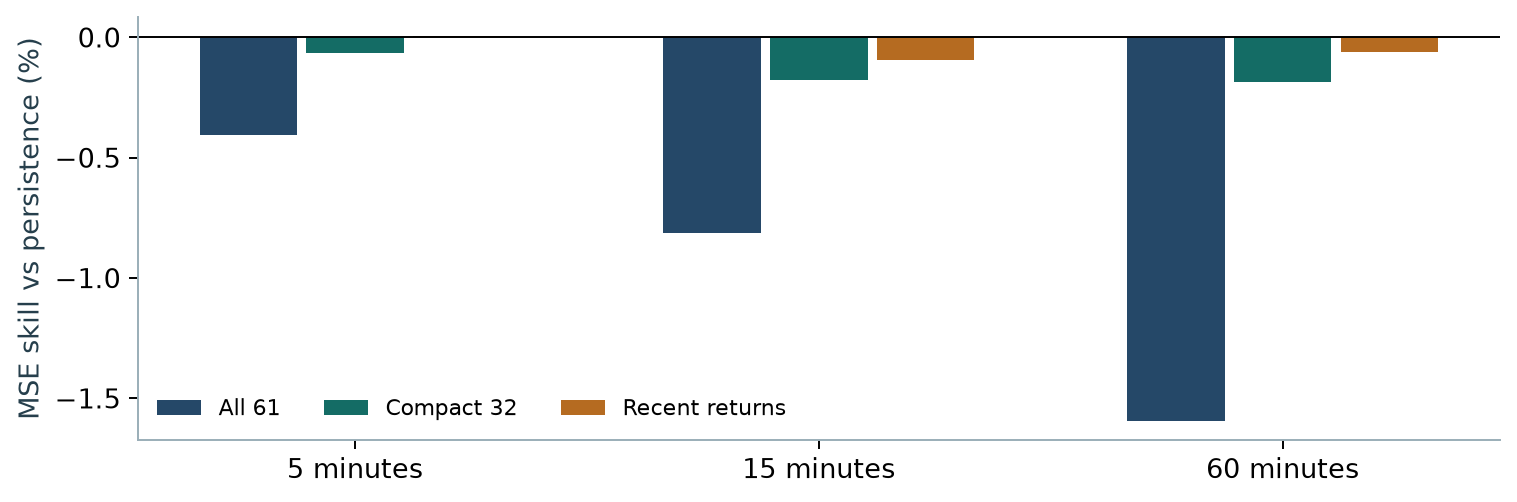
\includegraphics[width=\linewidth,height=51mm,keepaspectratio]{figures/7-skill.png}\par}
{\small\itshape Figure 6. Error reduction relative to predicting unchanged price. Zero denotes the persistence baseline. At 15 minutes, skill improved from -0.813\% to -0.177\% after feature reduction.\par}
The compact set improved on the full set at all three horizons, yet both remained below persistence on average. This result concerns the linear index experiment. The minute-level equity LSTM used a different target horizon and feature subset.\par
\clearpage
\section*{6. Trading the intraday LSTM forecasts}
\begin{itemize}\item \textbf{Prediction task.} Use 30 consecutive one-minute bars to predict the next bar's simple return. The seven features are simple return, log return, RSI(14), 20-bar percentage trend slope, 30-bar rolling volatility, 20-bar relative volume and log volume. Windows stay inside a continuous segment.\end{itemize}
\begin{itemize}\item \textbf{Training.} An 80/10/10 chronological split keeps whole sessions together. Adam optimizes the magnitude-weighted loss. The equity run adds extra weight when absolute returns reach 0.005, equivalent to a 0.5\% one-bar move.\end{itemize}
\begin{itemize}\item \textbf{Threshold policy.} Seek a long position when the predicted return exceeds 0.0001 (one basis point). The environment charges 0.00005 per side by default, so an entry and exit together cost about one basis point before execution effects.\end{itemize}
\begin{itemize}\item \textbf{Q-learning policy.} The state combines a forecast bucket, current position and one of three time-of-day buckets. Out-of-fold forecasts from earlier training windows supply policy experience; validation returns select the policy used on the test period.\end{itemize}
\begin{tabularx}{\linewidth}{@{}p{0.34\linewidth}XXXX@{}}\toprule
Stock & Threshold trades & Threshold P\&L & Q trades & Q P\&L\\\midrule
ADANIGREEN & 230 & -2,801.58 & 0 & 0.00\\
HYUNDAI & 337 & +34.04 & 340 & -3.54\\
LTIM & 224 & +52.04 & 224 & -1,334.78\\
RELIANCE & 26 & -188.86 & 44 & +47.24\\
\bottomrule\end{tabularx}\par
{\centering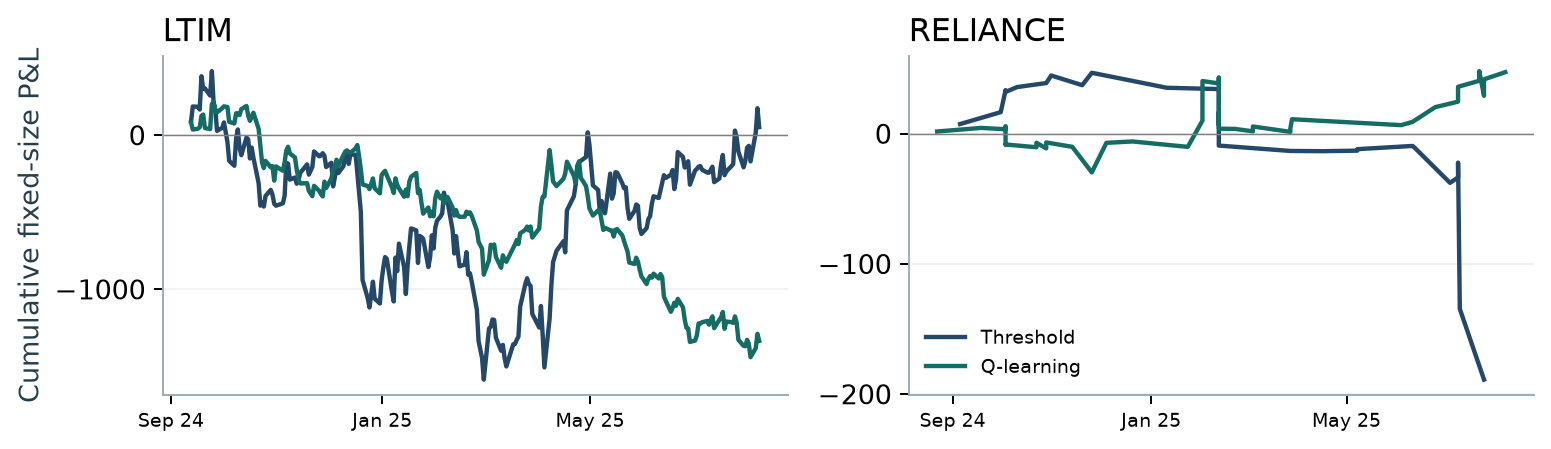
\includegraphics[width=\linewidth,height=46mm,keepaspectratio]{figures/8-paired-trades.png}\par}
{\small\itshape Figure 7. Cumulative net P\&L from the matched LTIM and RELIANCE logs. Each curve advances at completed trade exits under its own policy.\par}
\subsection*{What the paired logs show}
\begin{itemize}\item \textbf{ADANIGREEN.} The learned policy stayed in cash while the threshold rule accumulated losses. Zero here means that the RL trade file contained no completed trades.\end{itemize}
\begin{itemize}\item \textbf{LTIM and RELIANCE.} On LTIM both policies completed 224 trades, yet their outcomes differed by 1,386.82. On RELIANCE the learned policy turned a loss into a gain. A change in the trade count alone cannot explain both outcomes.\end{itemize}
The P\&L columns sum the logged net result per 10,000 of trade notional. They measure fixed-size trade outcomes. The portfolio experiments that follow use shared cash and report compounded account returns.\par
\clearpage
\section*{7. Parameter search and genetic programming}
The daily forex experiment evolved numeric trading parameters. The equity pipeline searches two different spaces: the settings of a predefined strategy and the structure of a trading rule.\par
\begin{tabularx}{\linewidth}{@{}p{0.26\linewidth}X@{}}\toprule
Equity strategy & What the search varies\\\midrule
VWAP mean reversion & VWAP window, deviation threshold and trend moving average\\
RSI mean reversion & RSI period, oversold level and overbought level\\
Bollinger reversion & Lookback period and band width\\
Donchian breakout & Lookback for the breakout channel\\
\bottomrule\end{tabularx}\par
\begin{itemize}\item \textbf{Parameter grid.} Each candidate is evaluated alongside stop distances of 0.50\%, 0.75\% and 1.00\%, and reward-to-risk ratios of 1, 2 or 3. A stop of 0.75\% paired with a ratio of 2 implies a 1.50\% target.\end{itemize}
\begin{itemize}\item \textbf{Genetic programming.} Leaves compare RSI or Bollinger position with a threshold. AND and OR nodes combine comparisons. The default search evolves 40 trees for 12 generations through tournament selection, subtree crossover and mutation. A per-node penalty discourages redundant conditions.\end{itemize}
\begin{itemize}\item \textbf{Walk-forward test.} The default schedule fits six past calendar months, freezes the selected rule for the next month, then advances by one month. A training winner can earn less than another candidate in the following evaluation month.\end{itemize}
{\centering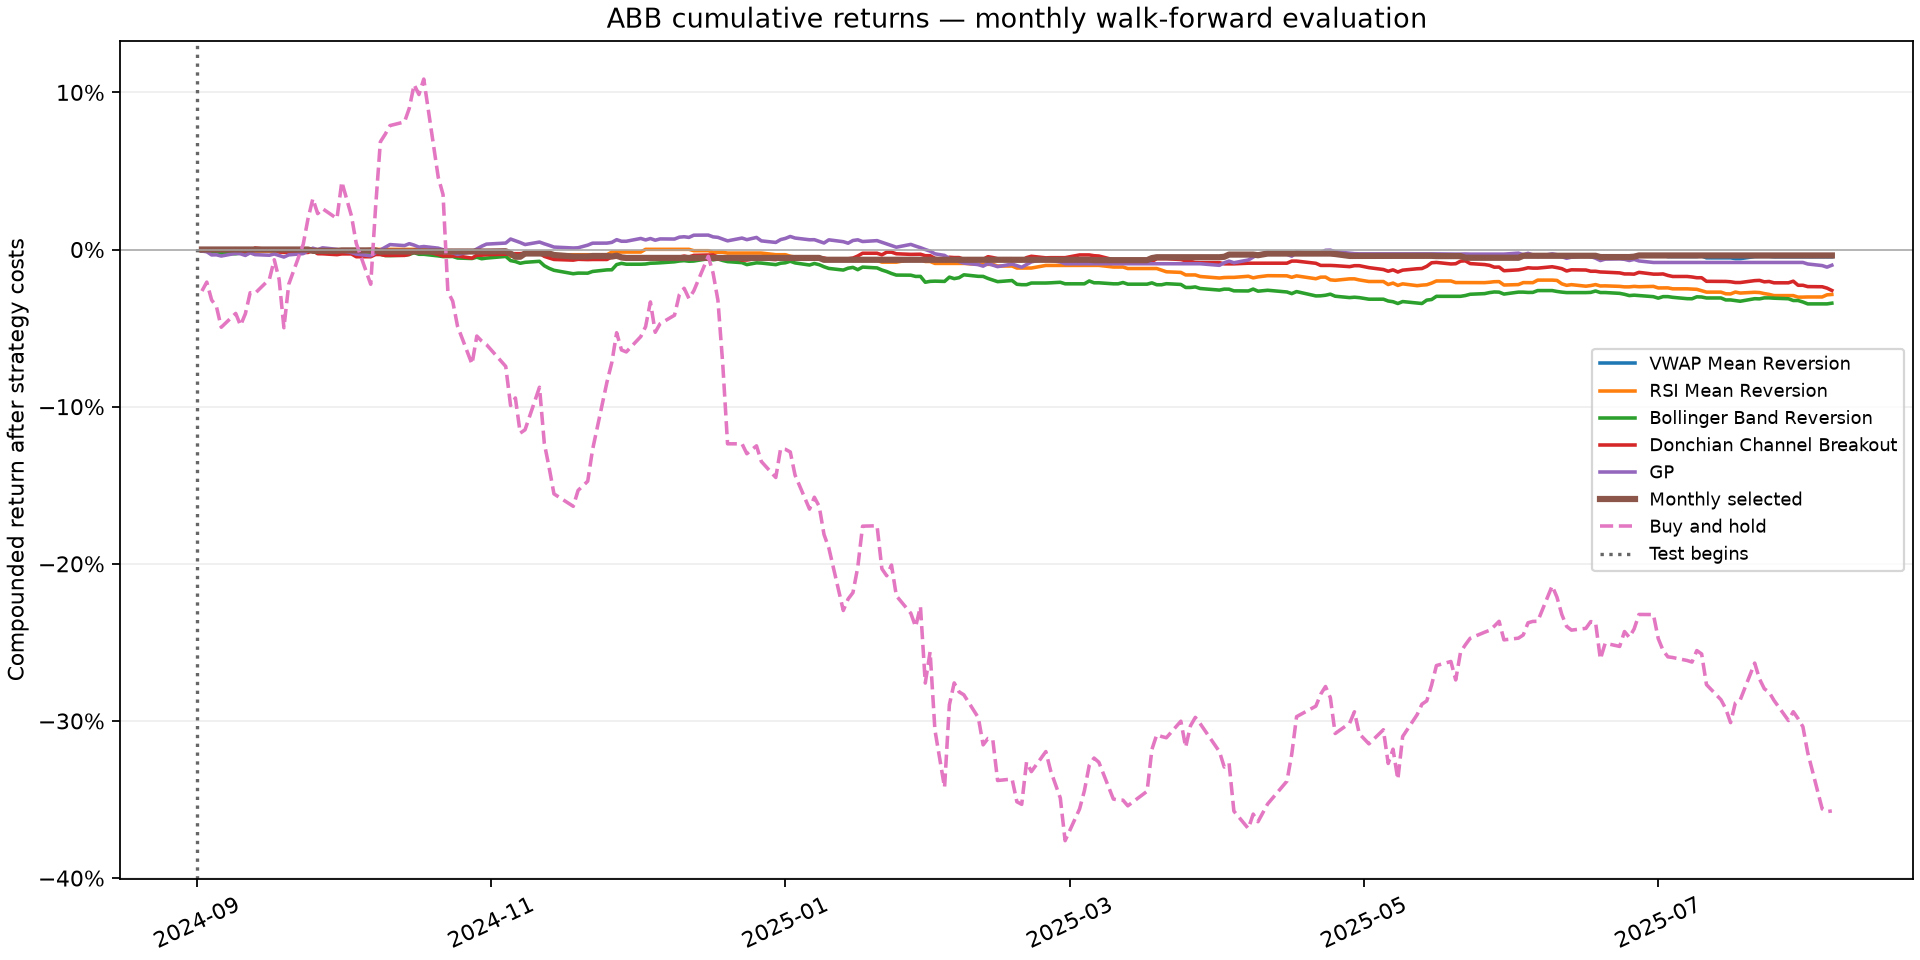
\includegraphics[width=\linewidth,height=60mm,keepaspectratio]{figures/9-ABB.png}\par}
{\small\itshape Figure 8. Saved ABB walk-forward comparison from the Calmar experiment. Each strategy and the monthly selected rule accumulate their own outcomes; the portfolio layer subsequently decides which stocks receive capital.\par}
\clearpage
\section*{8. Indian equity portfolio}
\begin{itemize}\item \textbf{Stock selection.} At each monthly rebalance the simulator ranks stocks by their selected strategy's compounded return over the preceding three complete months. The current evaluation month is excluded from that ranking.\end{itemize}
\begin{itemize}\item \textbf{Shared account.} Eligible signals compete for cash. Orders use whole shares. Strategy scoring uses observed closes, while the portfolio replay uses next-open execution rules and can defer exits. The portfolio curve therefore cannot be recovered by simply averaging stock-level returns.\end{itemize}
\begin{tabularx}{\linewidth}{@{}p{0.34\linewidth}XX@{}}\toprule
1 Dec 2020--6 Aug 2025 & Top 10 & Top 20\\\midrule
Allocation per entry & 12\% & 10\%\\
Cumulative return & +250.87\% & +104.85\%\\
Maximum daily drawdown & -19.83\% & -24.73\%\\
Executed fills & 45,872 & 50,210\\
\bottomrule\end{tabularx}\par
{\centering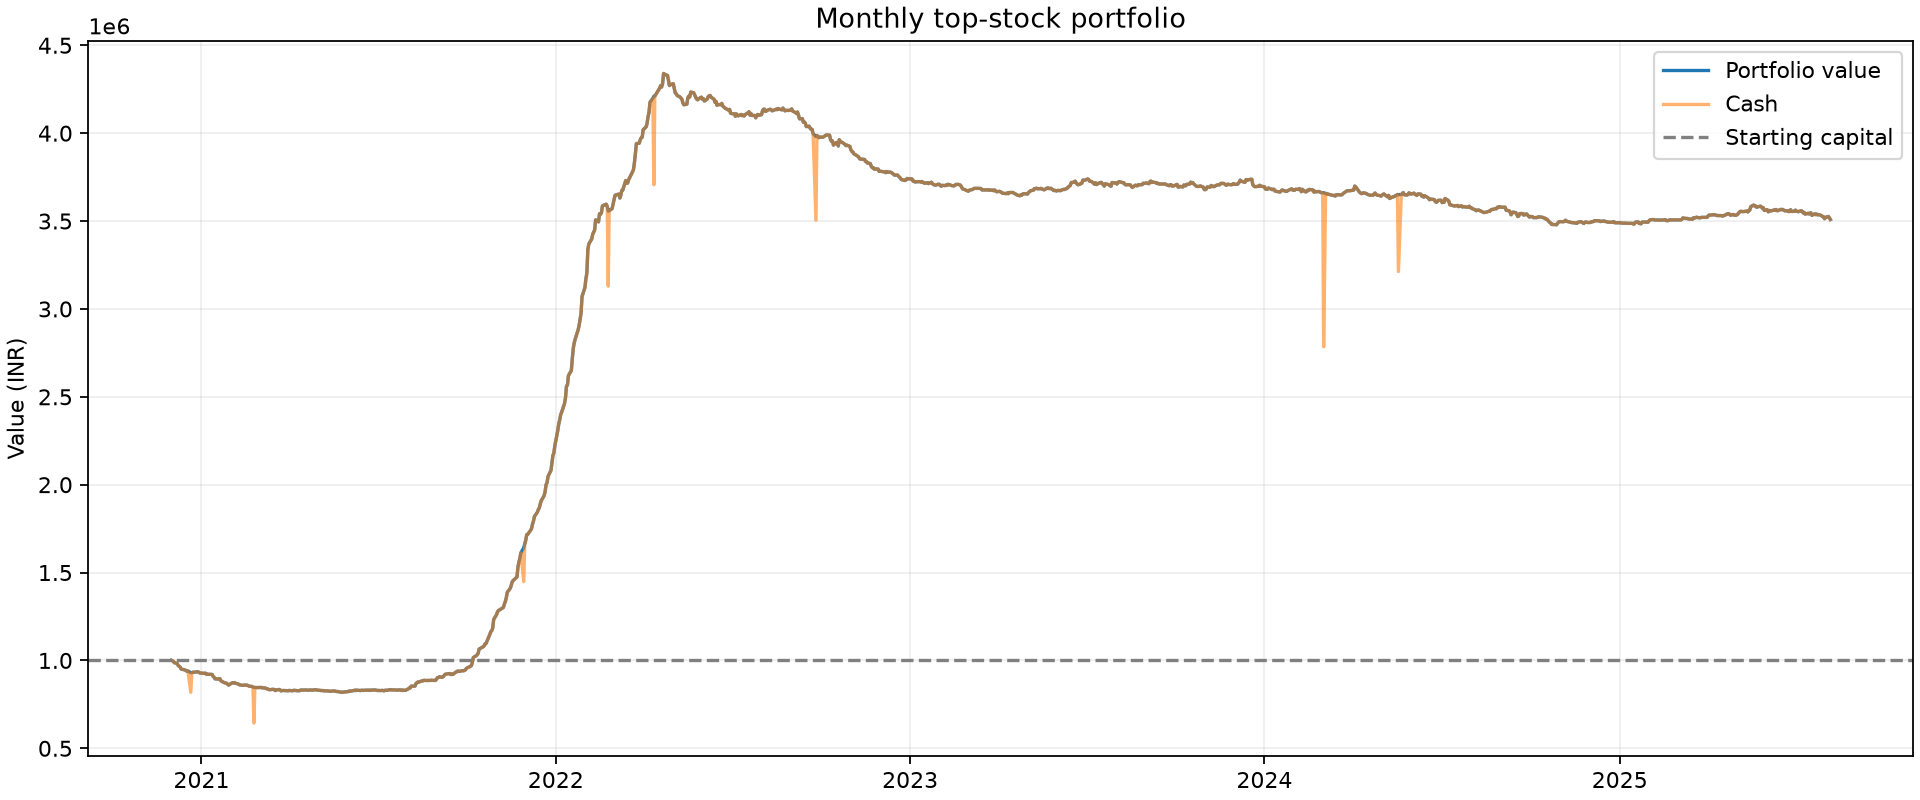
\includegraphics[width=\linewidth,height=77mm,keepaspectratio]{figures/10-portfolio_value.png}\par}
{\small\itshape Figure 9. Shared-capital Indian top-10 replay. The account rose from INR 1,000,000 to INR 3,508,725.13, with a maximum daily peak-to-trough decline of 19.83\%.\par}
\begin{itemize}\item \textbf{Costs.} The selected run recorded INR 3,419,384.13 in cumulative modeled fees over repeated turnover. Those charges are already reflected in ending equity. The fee model applies an encoded tariff scenario to the historical period.\end{itemize}
\begin{itemize}\item \textbf{Interpretation.} The top-10 run had the higher return and smaller daily drawdown. It also allocated more per entry. These runs do not isolate the effect of choosing ten stocks rather than twenty.\end{itemize}
\clearpage
\section*{9. US equity portfolio}
The US replay uses a three-month stock-ranking lookback, shared capital of USD 100,000 and a 5$\times$ leverage setting. Both portfolio-size runs use 10\% notional allocation. This setting limits entry notional as a share of equity; the leverage parameter governs margin funding.\par
\begin{tabularx}{\linewidth}{@{}p{0.34\linewidth}XX@{}}\toprule
1 May 2025--12 Nov 2026 & Top 10 & Top 20\\\midrule
Starting equity & 100,000.00 & 100,000.00\\
Ending equity & 108,923.13 & 112,499.25\\
Cumulative return & +8.92\% & +12.50\%\\
Maximum daily drawdown & -1.46\% & -1.20\%\\
Fills / recorded fees & 8,438 / 1,277.16 & 13,764 / 2,223.42\\
\bottomrule\end{tabularx}\par
{\centering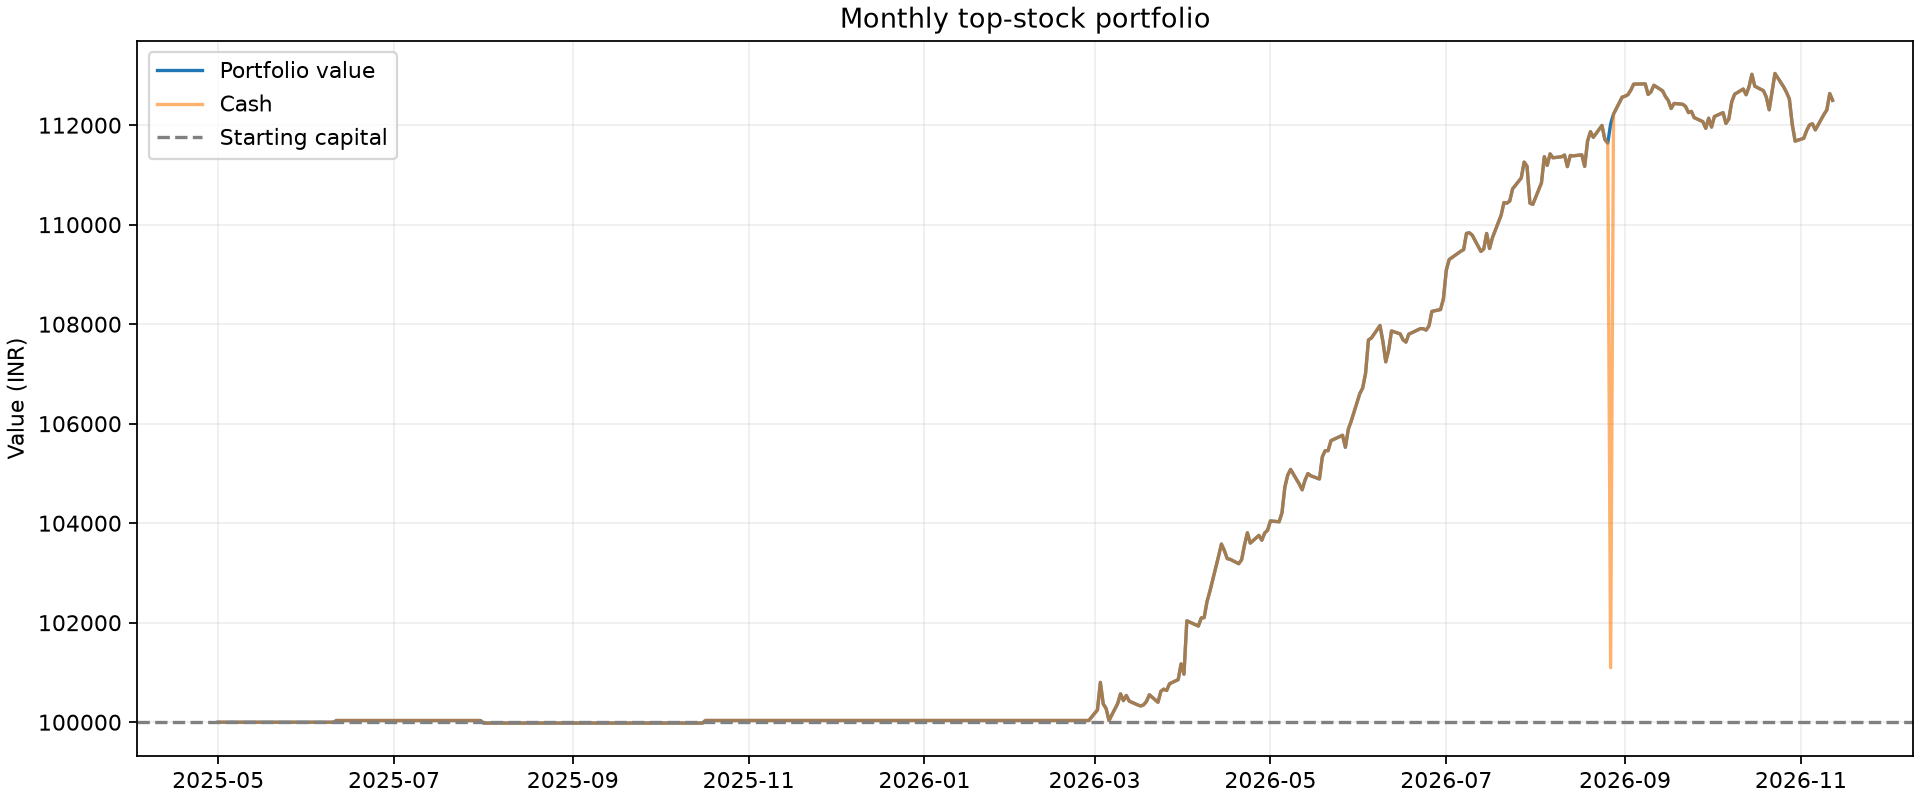
\includegraphics[width=\linewidth,height=70mm,keepaspectratio]{figures/11-portfolio_value.png}\par}
{\small\itshape Figure 10. US top-20 replay. On the same dates and nominal allocation, it returned 3.58 percentage points more than the top-10 run.\par}
\begin{itemize}\item \textbf{Execution record.} The top-20 ledger reports one overnight stock-day and zero margin events. Each fill is an executed order; a round trip normally generates both an entry and an exit.\end{itemize}
\begin{itemize}\item \textbf{Fee attribution.} The engine puts SEC and FINRA charges into legacy fields named sebi and ipft. The summary also has nonzero charge categories that the US fee function sets to zero. The return above reflects the recorded ledger; exchange-specific attribution remains unresolved.\end{itemize}
\clearpage
\section*{9.1 Shared portfolios versus buy-and-hold}
India: 1 December 2020 to 6 August 2025. US: 1 May 2025 to 12 November 2026. Within each market, the active portfolios and passive benchmark are measured over the same calendar period.\par
\begin{tabular*}{\linewidth}{@{\extracolsep{\fill}}lrrrr@{}}\toprule
Portfolio & India return & Excess (pp) & US return & Excess (pp)\\\midrule
Equal-money buy-and-hold & +220.97\% & - & +40.97\% & -\\
Top 10 & +250.87\% & +29.90 & +8.92\% & -32.04\\
Top 20 & +104.85\% & -116.12 & +12.50\% & -28.47\\
\bottomrule\end{tabular*}\par
Excess return is the active return less the passive return, in percentage points (pp), calculated before rounding.\par
\subsection*{India}
INR 10 lakh grew to INR 32.10 lakh by holding, INR 35.09 lakh with the top 10, and INR 20.48 lakh with the top 20. Only the top 10 beat holding. Its maximum daily drawdown was 19.83\%. Ending equity includes INR 34.19 lakh in modeled fees over 45,872 fills. The top 10 allocated 12\% per entry and the top 20 allocated 10\%, so the comparison also reflects position sizing.\par
\subsection*{United States}
USD 100,000 grew to approximately USD 140,967 by holding, USD 108,923 with the top 10, and USD 112,499 with the top 20. Both active portfolios earned a profit and trailed holding. The saved fee ledger contains nonzero charge categories that require reconciliation.\par
Benchmark construction: split starting capital equally across the saved universe, allow fractional shares and hold without rebalancing. Seven Indian allocations stayed in cash until their first valid bar. One US holding was valued at its last valid close. The calculation uses recorded prices with no added dividends or passive trading fees. Corporate-action adjustments and historical universe membership have not been independently verified.\par
\clearpage
\section*{9.2 Trading charges in the Indian and US top-10 portfolios}
For a strategy that repeatedly buys and sells, the relevant hurdle is the fee per unit traded. On the recorded fills, an Indian round trip required about 5.21 basis points of price improvement to cover explicit charges. The US replay required 0.29 basis points under its zero-commission assumption. One basis point is 0.01\%.
\begin{tabularx}{\linewidth}{@{}Xrr@{}}\toprule
Recorded measure & India (INR) & US (USD)\\\midrule
Buy plus sell turnover & 13,133,724,706 & 88,718,955\\
Explicit fees & 3,419,384 & 1,277\\
Trading profit before recorded fees & 5,928,109 & 10,200\\
Profit after recorded fees & 2,508,725 & 8,923\\
Share of pre-fee profit consumed & 57.68\% & 12.52\%\\
Round-trip fee equivalent & 5.21 bp & 0.29 bp\\\bottomrule
\end{tabularx}
\subsection*{Which Indian charges mattered most?}
\begin{itemize}
\item Securities transaction tax accounted for INR 1,648,094 (48.2\% of fees). Brokerage added INR 917,440 (26.8\%). Together they accounted for three quarters of the bill.
\item Exchange charges contributed INR 403,191, GST INR 240,103 and stamp duty INR 197,305. Regulatory and depository charges made up the remainder.
\end{itemize}
\subsection*{What a small trading edge would retain}
At the observed turnover mix, a signal earning 4 bp gross per round trip would lose about 1.21 bp in India and retain 3.71 bp in the US replay before spread and slippage. The Indian strategy itself remained profitable after fees. The two portfolios traded different stocks on different dates with different sizing, so their returns cannot isolate a country effect.
\par\smallskip
{\small Method and sources. Turnover sums shares times fill price across buys and sells in each top-10 executed-trades ledger. Round-trip equivalent equals 20,000 times total fees divided by turnover. Pre-fee profit adds recorded fees back to net profit with fills held fixed. The Indian replay applies the saved FYERS tariff scenario to historical trades. The US replay models zero brokerage and regulatory fees. Actual US commissions depend on broker plan and eligibility. Sources: the two top-10 summary.json files and their executed\_trades.csv ledgers.}
\clearpage
\section*{10. Reinforcement learning over strategy signals}
\begin{itemize}\item \textbf{Observations.} The final policy sees four technical strategy signals, the GP signal, price information relative to the previous close, position status, cash and time of day. A shared network chooses HOLD, BUY or SELL-to-close for each available stock.\end{itemize}
\begin{itemize}\item \textbf{Execution.} Decisions made at the close execute at the next eligible open. Shared cash couples decisions across the 95 stocks. The drawdown-aware run allocates 4\% per entry and limits the portfolio to ten open positions.\end{itemize}
\begin{itemize}\item \textbf{Learning.} The actor--critic update combines discounted rewards, a value estimate and entropy regularization. Each step rewards log equity growth and penalizes increases in drawdown. The saved run starts training in December 2025 and selects among five epochs using validation return plus signed maximum drawdown.\end{itemize}
\begin{tabularx}{\linewidth}{@{}p{0.34\linewidth}XX@{}}\toprule
Drawdown-aware policy & Validation & Held-out test\\\midrule
Period & Jun--Aug 2026 & 1 Sep--12 Nov 2026\\
Cumulative return & +4.00\% & +4.02\%\\
Maximum drawdown & -1.76\% & -1.38\%\\
Fills / fees (USD) & 1,280 / 70.95 & 1,040 / 57.03\\
\bottomrule\end{tabularx}\par
{\centering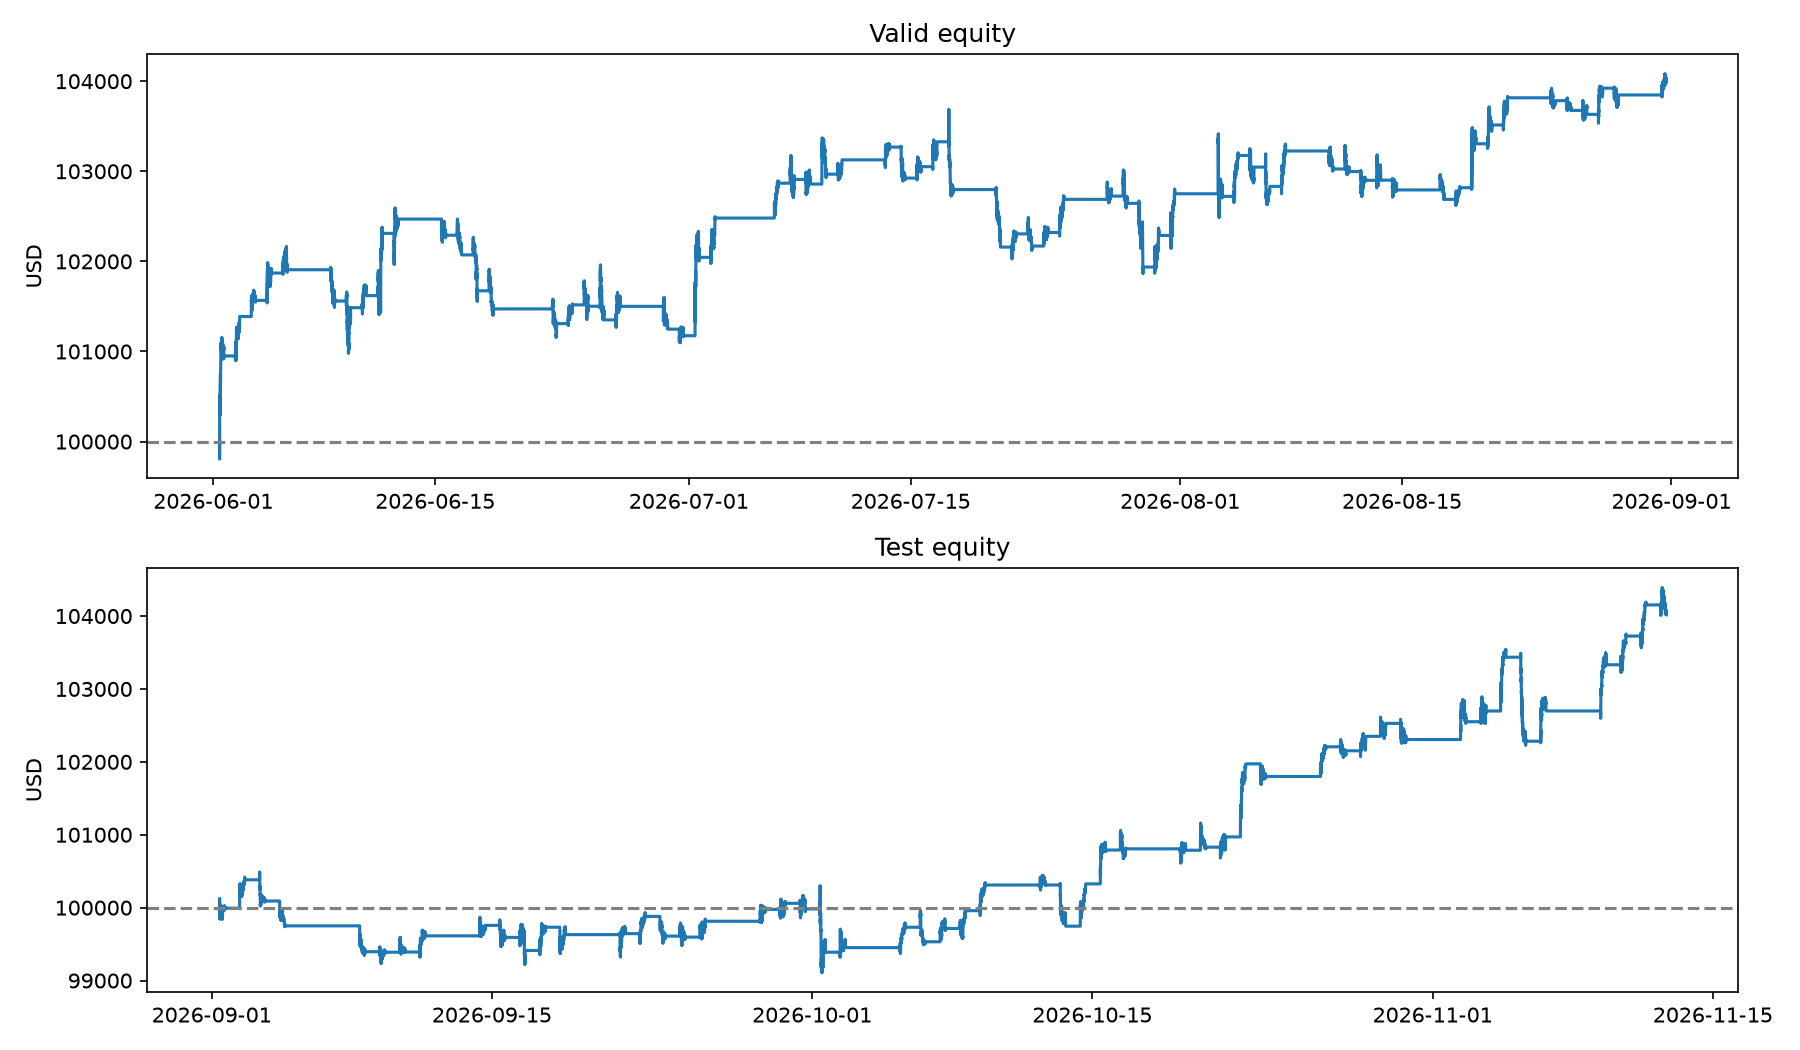
\includegraphics[width=\linewidth,height=61mm,keepaspectratio]{figures/12-equity.png}\par}
{\small\itshape Figure 11. Saved validation and test equity curves. The test started at USD 100,000 and ended at USD 104,016.35. Each panel begins with its own starting capital.\par}
A separate 95-stock policy stayed in cash throughout validation and test. The active policy beat that zero-return reference on the held-out period. Establishing an advantage over the top-20 rules portfolio requires a replay on matching dates with matching exposure limits.\par
\clearpage
\clearpage
\section*{11. Future Plans}
The open questions from Section~12 suggest three concrete next experiments and one theoretical extension.
\begin{itemize}
  \item \textbf{Central bank intervention modelling.} RBI and ECB intervention events trigger large sudden price moves that existing models treat as random noise. Parsing central bank meeting minutes and intervention announcements with language models could add a leading signal for regime changes in EUR/USD and USD/INR, addressing the data-scarcity gap identified in the literature review.
  \item \textbf{SHAP explainability on LSTM hidden states.} Applying SHAP values to the LSTM's hidden state at each forecast step would identify which of the 23 macro and technical features most influenced each prediction. This would address the second gap from the literature review: post hoc analysis of which macro variables drive RL and LSTM decisions during specific market events such as FOMC announcements or RBI rate changes.
  \item \textbf{Controlled loss-function ablation.} BigMoveAwareLoss is the central design choice of the daily forecasting work, but no controlled comparison against standard MSE has been run on a fixed seed and fixed split. Running three seeds each for plain MSE, magnitude weighting only, and the full BigMoveAwareLoss would isolate the contribution of each component and determine whether the sign-mismatch penalty adds value beyond the magnitude upweighting.
  \item \textbf{Extending portfolio RL to Indian equities.} The actor--critic policy in Section~10 was trained and tested on 95 US stocks. Applying the same framework to the 100-stock Indian universe, with the FYERS fee schedule, would test whether the RL layer adds value over the rule-based portfolio in a higher-cost market where the fee breakeven per round trip is 5.21 basis points.
\end{itemize}
\clearpage
\section*{12. Conclusions and next experiments}
\subsection*{What each experiment established}
\begin{itemize}\item \textbf{Forecasting.} On 681 test observations the USD/INR LSTM gained three correct calls over always-up. Fine-tuning EUR/USD increased correct predictions by 16. Both daily index directional scores were below 50\%.\end{itemize}
\begin{itemize}\item \textbf{Execution.} In the 65-session EUR/USD simulation, average wins exceeded average losses. The resulting +2.28\% account return exceeded the exact passive EUR reference by 3.87 percentage points despite a trade win rate below 50\%.\end{itemize}
\begin{itemize}\item \textbf{Data quality.} Distinguishing exchange closures, incomplete histories and intraday gaps changed which windows qualified for forecasting. The retrospective short-gap rule and continuous-segment checks make preprocessing part of the experimental design.\end{itemize}
\begin{itemize}\item \textbf{Trading policy.} A single-stock forecast policy reduced losses for ADANIGREEN and improved RELIANCE, but performed much worse on LTIM. The later portfolio policy using five strategy signals returned 4.02\% in one held-out US period.\end{itemize}
\subsection*{Comparisons that would resolve the open questions}
\begin{tabularx}{\linewidth}{@{}p{0.26\linewidth}X@{}}\toprule
Question & Controlled experiment\\\midrule
Does the loss improve direction? & Fix the LSTM, seed and chronological split. Compare squared error, magnitude weighting and a differentiable direction penalty.\\
How much does gap repair matter? & Compare observed-only windows, causal repair and two-sided repair on the same eligible target timestamps.\\
Does portfolio RL add value? & Replay cash, the underlying strategy rules and RL on 1 Sep--12 Nov 2026 using identical capital, stock eligibility and exposure limits.\\
How sensitive are returns to costs? & Reconcile the US fee ledger and rerun with common spread and slippage assumptions. Evaluate frozen configurations on later months and multiple training seeds.\\
\bottomrule\end{tabularx}\par
\clearpage
\section*{References and experimental records}
\subsection*{Research references}
[1] M. Fisichella and F. Garolla. Can Deep Learning Improve Technical Analysis of Forex Data to Predict Future Price Movements? IEEE Access, 2021. DOI 10.1109/ACCESS.2021.3127570.\par
[2] C.-Y. Huang. Financial Trading as a Game: A Deep Reinforcement Learning Approach. arXiv:1807.02787, 2018. The sequential-decision formulation motivates using position and cash as policy inputs.\par
[3] P. Babu and N. Geethanjali. FOREX Trend Classification using Machine Learning Techniques. International Journal of Computer Applications, 2011.\par
[4] R. Sharma and K. C. Pradhan. Macro-Quant: A Hybrid Machine Learning Framework for Non-Stationary Exchange Rate Forecasting. Journal of Financial Econometrics, 2025.\par
[5] G. Giacinto et al. Deep LSTM with Reinforcement Learning Layer for Financial Trend Prediction in FX High Frequency Trading Systems. Applied Soft Computing, 2019.\par
[6] S. Grover et al. An Ensembling Architecture Incorporating Machine Learning Models and Genetic Algorithm Optimization for Forex Trading. Expert Systems with Applications, 2022.\par
\subsection*{Where to reproduce the reported results}
\begin{itemize}\item \textbf{Daily models.} The earlier report and presentation document the original experiments. train.ipynb contains the baseline and LSTM runs. evaluate.ipynb compares model outputs. Corrected directional scores use the saved model\_results.json predictions, FRED series and held-out index prediction CSVs in runs/.\end{itemize}
\begin{itemize}\item \textbf{EUR/USD benchmark.} run\_2026.py updates the passive euro account from daily EUR/USD log returns. reports/real\_trading\_2026/simulation\_2026\_trades.csv contains both daily account paths. The companion simulation\_2026\_metrics.json contains the original benchmark, win/loss counts and annualization.\end{itemize}
\begin{itemize}\item \textbf{Equity data.} full\_predictor/eda/eda.ipynb and eda\_outputs contain calendar, coverage and missing-run audits. helpers/feature\_engineering.py implements gap repair, indicator resets and daily GARCH. reports/indicator\_analysis contains the separate five-minute ridge screen.\end{itemize}
\begin{itemize}\item \textbf{Intraday LSTM.} full\_predictor/main.py, loss\_functions.py, models.py and rl\_model.py define the regressor and Q-learning experiment. The four paired threshold and RL trade logs under full\_predictor/reports supply the fixed-size P\&L comparison.\end{itemize}
\begin{itemize}\item \textbf{Equity strategy search.} full\_predictor/GA\_STRATEGY contains the strategy grids, GP optimizer, monthly batch runner, execution code and portfolio replay. Each selected portfolio directory includes a summary, daily account values, charges, stock rankings and trade ledger.\end{itemize}
\begin{itemize}\item \textbf{Portfolio RL.} full\_predictor/rl agent contains the market environment and trainer. The rl\_us\_all\_drawdown and rl\_us\_all\_run2 directories contain configurations, validation and test logs and policy checkpoints.\end{itemize}
\end{document}